% Created by tikzDevice version 0.12 on 2019-02-10 18:18:55
% !TEX encoding = UTF-8 Unicode
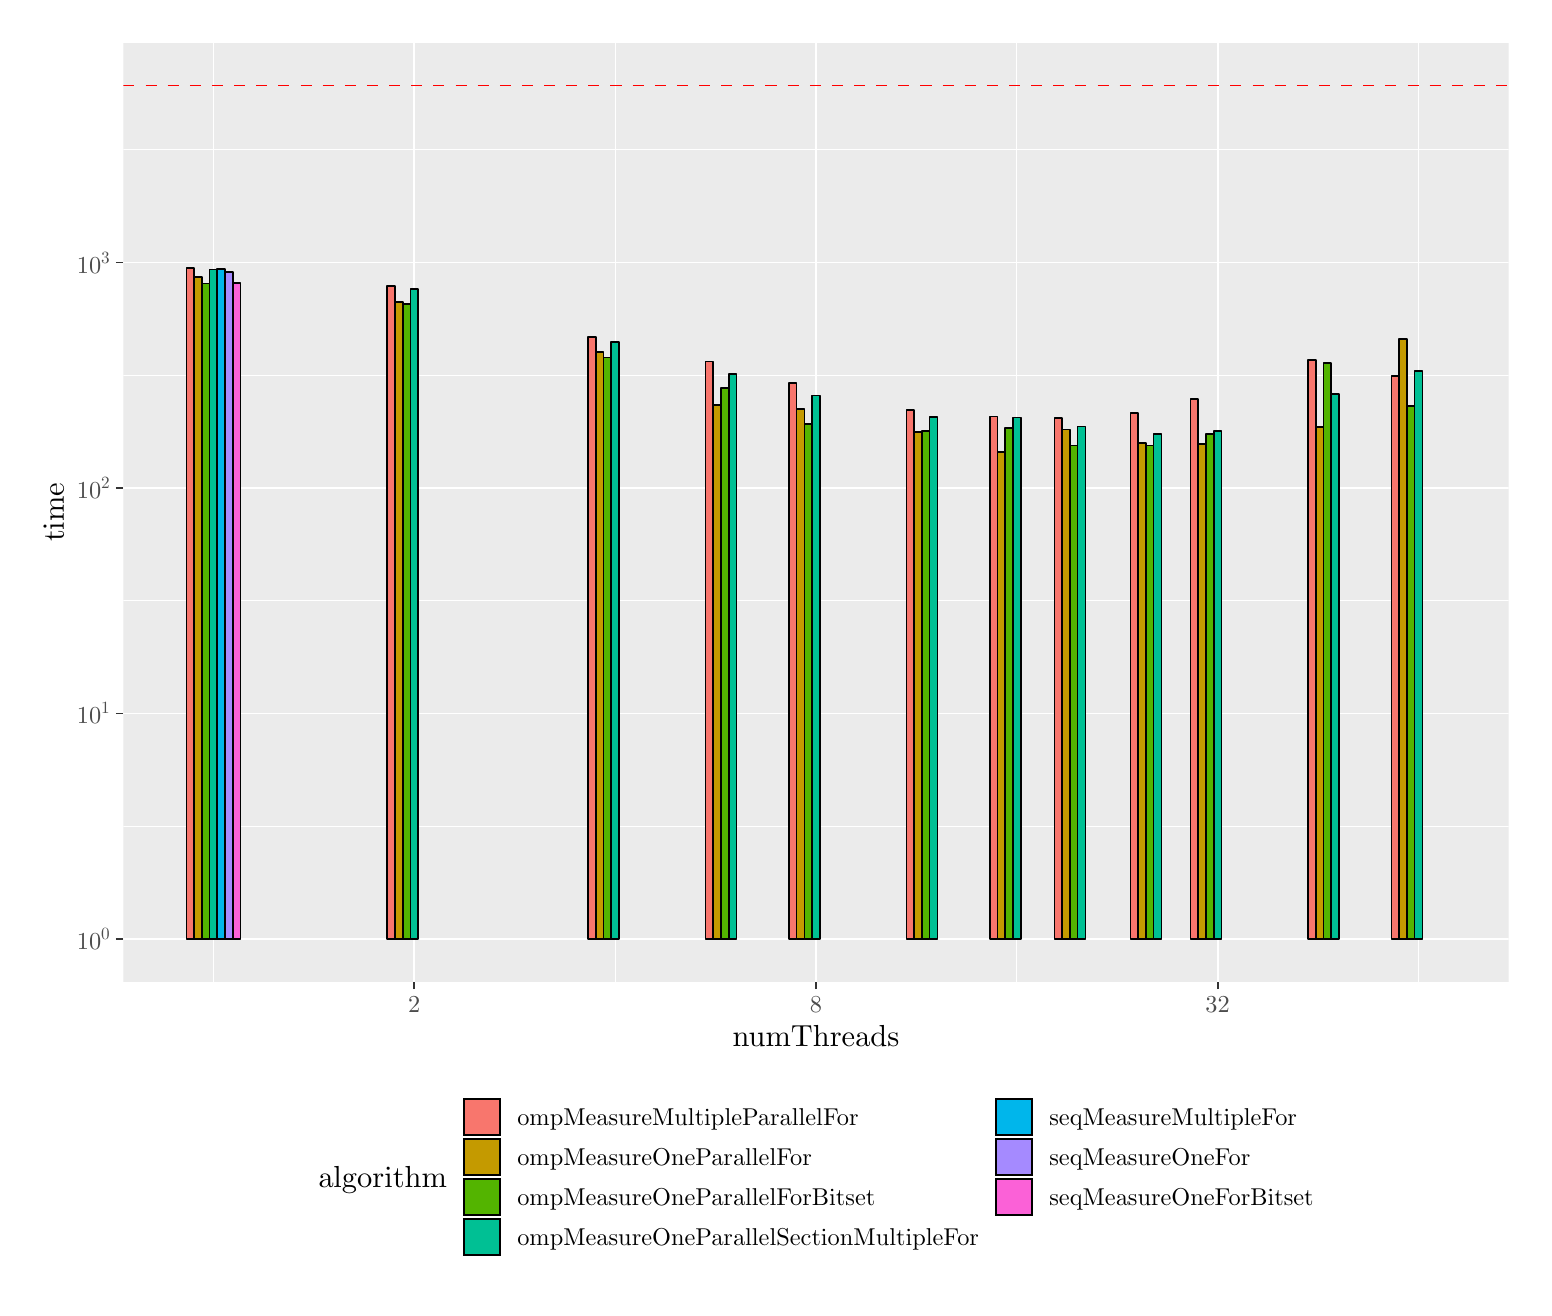
\begin{tikzpicture}[x=1pt,y=1pt]
\definecolor{fillColor}{RGB}{255,255,255}
\path[use as bounding box,fill=fillColor,fill opacity=0.00] (0,0) rectangle (540.60,455.24);
\begin{scope}
\path[clip] (  0.00,  0.00) rectangle (540.60,455.24);
\definecolor{drawColor}{RGB}{255,255,255}
\definecolor{fillColor}{RGB}{255,255,255}

\path[draw=drawColor,line width= 0.6pt,line join=round,line cap=round,fill=fillColor] (  0.00,  0.00) rectangle (540.60,455.24);
\end{scope}
\begin{scope}
\path[clip] ( 34.60,110.54) rectangle (535.10,449.74);
\definecolor{fillColor}{gray}{0.92}

\path[fill=fillColor] ( 34.60,110.54) rectangle (535.10,449.74);
\definecolor{drawColor}{RGB}{255,255,255}

\path[draw=drawColor,line width= 0.3pt,line join=round] ( 34.60,166.69) --
	(535.10,166.69);

\path[draw=drawColor,line width= 0.3pt,line join=round] ( 34.60,248.16) --
	(535.10,248.16);

\path[draw=drawColor,line width= 0.3pt,line join=round] ( 34.60,329.63) --
	(535.10,329.63);

\path[draw=drawColor,line width= 0.3pt,line join=round] ( 34.60,411.10) --
	(535.10,411.10);

\path[draw=drawColor,line width= 0.3pt,line join=round] ( 67.13,110.54) --
	( 67.13,449.74);

\path[draw=drawColor,line width= 0.3pt,line join=round] (212.28,110.54) --
	(212.28,449.74);

\path[draw=drawColor,line width= 0.3pt,line join=round] (357.42,110.54) --
	(357.42,449.74);

\path[draw=drawColor,line width= 0.3pt,line join=round] (502.57,110.54) --
	(502.57,449.74);

\path[draw=drawColor,line width= 0.6pt,line join=round] ( 34.60,125.96) --
	(535.10,125.96);

\path[draw=drawColor,line width= 0.6pt,line join=round] ( 34.60,207.43) --
	(535.10,207.43);

\path[draw=drawColor,line width= 0.6pt,line join=round] ( 34.60,288.90) --
	(535.10,288.90);

\path[draw=drawColor,line width= 0.6pt,line join=round] ( 34.60,370.36) --
	(535.10,370.36);

\path[draw=drawColor,line width= 0.6pt,line join=round] (139.70,110.54) --
	(139.70,449.74);

\path[draw=drawColor,line width= 0.6pt,line join=round] (284.85,110.54) --
	(284.85,449.74);

\path[draw=drawColor,line width= 0.6pt,line join=round] (430.00,110.54) --
	(430.00,449.74);
\definecolor{drawColor}{RGB}{0,0,0}
\definecolor{fillColor}{RGB}{251,97,215}

\path[draw=drawColor,line width= 0.6pt,line join=round,fill=fillColor] ( 74.12,125.96) rectangle ( 76.91,362.92);
\definecolor{fillColor}{RGB}{165,138,255}

\path[draw=drawColor,line width= 0.6pt,line join=round,fill=fillColor] ( 71.32,125.96) rectangle ( 74.12,366.86);
\definecolor{fillColor}{RGB}{0,182,235}

\path[draw=drawColor,line width= 0.6pt,line join=round,fill=fillColor] ( 68.53,125.96) rectangle ( 71.32,368.11);
\definecolor{fillColor}{RGB}{0,192,148}

\path[draw=drawColor,line width= 0.6pt,line join=round,fill=fillColor] ( 65.73,125.96) rectangle ( 68.53,367.83);
\definecolor{fillColor}{RGB}{83,180,0}

\path[draw=drawColor,line width= 0.6pt,line join=round,fill=fillColor] ( 62.94,125.96) rectangle ( 65.73,362.84);
\definecolor{fillColor}{RGB}{196,154,0}

\path[draw=drawColor,line width= 0.6pt,line join=round,fill=fillColor] ( 60.14,125.96) rectangle ( 62.94,365.12);
\definecolor{fillColor}{RGB}{248,118,109}

\path[draw=drawColor,line width= 0.6pt,line join=round,fill=fillColor] ( 57.35,125.96) rectangle ( 60.14,368.45);
\definecolor{fillColor}{RGB}{0,192,148}

\path[draw=drawColor,line width= 0.6pt,line join=round,fill=fillColor] (138.31,125.96) rectangle (141.10,360.77);
\definecolor{fillColor}{RGB}{83,180,0}

\path[draw=drawColor,line width= 0.6pt,line join=round,fill=fillColor] (135.51,125.96) rectangle (138.31,355.43);
\definecolor{fillColor}{RGB}{196,154,0}

\path[draw=drawColor,line width= 0.6pt,line join=round,fill=fillColor] (132.72,125.96) rectangle (135.51,356.20);
\definecolor{fillColor}{RGB}{248,118,109}

\path[draw=drawColor,line width= 0.6pt,line join=round,fill=fillColor] (129.92,125.96) rectangle (132.72,361.88);
\definecolor{fillColor}{RGB}{0,192,148}

\path[draw=drawColor,line width= 0.6pt,line join=round,fill=fillColor] (210.88,125.96) rectangle (213.67,341.72);
\definecolor{fillColor}{RGB}{83,180,0}

\path[draw=drawColor,line width= 0.6pt,line join=round,fill=fillColor] (208.08,125.96) rectangle (210.88,336.03);
\definecolor{fillColor}{RGB}{196,154,0}

\path[draw=drawColor,line width= 0.6pt,line join=round,fill=fillColor] (205.29,125.96) rectangle (208.08,337.98);
\definecolor{fillColor}{RGB}{248,118,109}

\path[draw=drawColor,line width= 0.6pt,line join=round,fill=fillColor] (202.49,125.96) rectangle (205.29,343.49);
\definecolor{fillColor}{RGB}{0,192,148}

\path[draw=drawColor,line width= 0.6pt,line join=round,fill=fillColor] (253.33,125.96) rectangle (256.13,330.05);
\definecolor{fillColor}{RGB}{83,180,0}

\path[draw=drawColor,line width= 0.6pt,line join=round,fill=fillColor] (250.54,125.96) rectangle (253.33,324.92);
\definecolor{fillColor}{RGB}{196,154,0}

\path[draw=drawColor,line width= 0.6pt,line join=round,fill=fillColor] (247.74,125.96) rectangle (250.54,318.83);
\definecolor{fillColor}{RGB}{248,118,109}

\path[draw=drawColor,line width= 0.6pt,line join=round,fill=fillColor] (244.95,125.96) rectangle (247.74,334.57);
\definecolor{fillColor}{RGB}{0,192,148}

\path[draw=drawColor,line width= 0.6pt,line join=round,fill=fillColor] (283.45,125.96) rectangle (286.25,322.31);
\definecolor{fillColor}{RGB}{83,180,0}

\path[draw=drawColor,line width= 0.6pt,line join=round,fill=fillColor] (280.66,125.96) rectangle (283.45,312.05);
\definecolor{fillColor}{RGB}{196,154,0}

\path[draw=drawColor,line width= 0.6pt,line join=round,fill=fillColor] (277.86,125.96) rectangle (280.66,317.39);
\definecolor{fillColor}{RGB}{248,118,109}

\path[draw=drawColor,line width= 0.6pt,line join=round,fill=fillColor] (275.07,125.96) rectangle (277.86,326.93);
\definecolor{fillColor}{RGB}{0,192,148}

\path[draw=drawColor,line width= 0.6pt,line join=round,fill=fillColor] (325.90,125.96) rectangle (328.70,314.45);
\definecolor{fillColor}{RGB}{83,180,0}

\path[draw=drawColor,line width= 0.6pt,line join=round,fill=fillColor] (323.11,125.96) rectangle (325.90,309.53);
\definecolor{fillColor}{RGB}{196,154,0}

\path[draw=drawColor,line width= 0.6pt,line join=round,fill=fillColor] (320.31,125.96) rectangle (323.11,309.13);
\definecolor{fillColor}{RGB}{248,118,109}

\path[draw=drawColor,line width= 0.6pt,line join=round,fill=fillColor] (317.52,125.96) rectangle (320.31,317.01);
\definecolor{fillColor}{RGB}{0,192,148}

\path[draw=drawColor,line width= 0.6pt,line join=round,fill=fillColor] (356.03,125.96) rectangle (358.82,314.43);
\definecolor{fillColor}{RGB}{83,180,0}

\path[draw=drawColor,line width= 0.6pt,line join=round,fill=fillColor] (353.23,125.96) rectangle (356.03,310.46);
\definecolor{fillColor}{RGB}{196,154,0}

\path[draw=drawColor,line width= 0.6pt,line join=round,fill=fillColor] (350.44,125.96) rectangle (353.23,302.02);
\definecolor{fillColor}{RGB}{248,118,109}

\path[draw=drawColor,line width= 0.6pt,line join=round,fill=fillColor] (347.64,125.96) rectangle (350.44,314.77);
\definecolor{fillColor}{RGB}{0,192,148}

\path[draw=drawColor,line width= 0.6pt,line join=round,fill=fillColor] (379.39,125.96) rectangle (382.18,311.17);
\definecolor{fillColor}{RGB}{83,180,0}

\path[draw=drawColor,line width= 0.6pt,line join=round,fill=fillColor] (376.59,125.96) rectangle (379.39,304.20);
\definecolor{fillColor}{RGB}{196,154,0}

\path[draw=drawColor,line width= 0.6pt,line join=round,fill=fillColor] (373.80,125.96) rectangle (376.59,310.05);
\definecolor{fillColor}{RGB}{248,118,109}

\path[draw=drawColor,line width= 0.6pt,line join=round,fill=fillColor] (371.00,125.96) rectangle (373.80,314.31);
\definecolor{fillColor}{RGB}{0,192,148}

\path[draw=drawColor,line width= 0.6pt,line join=round,fill=fillColor] (406.86,125.96) rectangle (409.65,308.38);
\definecolor{fillColor}{RGB}{83,180,0}

\path[draw=drawColor,line width= 0.6pt,line join=round,fill=fillColor] (404.06,125.96) rectangle (406.86,304.27);
\definecolor{fillColor}{RGB}{196,154,0}

\path[draw=drawColor,line width= 0.6pt,line join=round,fill=fillColor] (401.27,125.96) rectangle (404.06,305.14);
\definecolor{fillColor}{RGB}{248,118,109}

\path[draw=drawColor,line width= 0.6pt,line join=round,fill=fillColor] (398.47,125.96) rectangle (401.27,316.01);
\definecolor{fillColor}{RGB}{0,192,148}

\path[draw=drawColor,line width= 0.6pt,line join=round,fill=fillColor] (428.60,125.96) rectangle (431.39,309.49);
\definecolor{fillColor}{RGB}{83,180,0}

\path[draw=drawColor,line width= 0.6pt,line join=round,fill=fillColor] (425.80,125.96) rectangle (428.60,308.41);
\definecolor{fillColor}{RGB}{196,154,0}

\path[draw=drawColor,line width= 0.6pt,line join=round,fill=fillColor] (423.01,125.96) rectangle (425.80,304.78);
\definecolor{fillColor}{RGB}{248,118,109}

\path[draw=drawColor,line width= 0.6pt,line join=round,fill=fillColor] (420.21,125.96) rectangle (423.01,320.95);
\definecolor{fillColor}{RGB}{0,192,148}

\path[draw=drawColor,line width= 0.6pt,line join=round,fill=fillColor] (471.05,125.96) rectangle (473.85,322.91);
\definecolor{fillColor}{RGB}{83,180,0}

\path[draw=drawColor,line width= 0.6pt,line join=round,fill=fillColor] (468.26,125.96) rectangle (471.05,334.12);
\definecolor{fillColor}{RGB}{196,154,0}

\path[draw=drawColor,line width= 0.6pt,line join=round,fill=fillColor] (465.46,125.96) rectangle (468.26,311.04);
\definecolor{fillColor}{RGB}{248,118,109}

\path[draw=drawColor,line width= 0.6pt,line join=round,fill=fillColor] (462.67,125.96) rectangle (465.46,335.12);
\definecolor{fillColor}{RGB}{0,192,148}

\path[draw=drawColor,line width= 0.6pt,line join=round,fill=fillColor] (501.17,125.96) rectangle (503.97,331.13);
\definecolor{fillColor}{RGB}{83,180,0}

\path[draw=drawColor,line width= 0.6pt,line join=round,fill=fillColor] (498.38,125.96) rectangle (501.17,318.62);
\definecolor{fillColor}{RGB}{196,154,0}

\path[draw=drawColor,line width= 0.6pt,line join=round,fill=fillColor] (495.58,125.96) rectangle (498.38,342.83);
\definecolor{fillColor}{RGB}{248,118,109}

\path[draw=drawColor,line width= 0.6pt,line join=round,fill=fillColor] (492.79,125.96) rectangle (495.58,329.39);
\definecolor{drawColor}{RGB}{255,0,0}

\path[draw=drawColor,line width= 0.6pt,dash pattern=on 4pt off 4pt ,line join=round] ( 34.60,434.33) -- (535.10,434.33);
\end{scope}
\begin{scope}
\path[clip] (  0.00,  0.00) rectangle (540.60,455.24);
\definecolor{drawColor}{gray}{0.30}

\node[text=drawColor,anchor=base west,inner sep=0pt, outer sep=0pt, scale=  0.88] at ( 17.77,122.18) {10};

\node[text=drawColor,anchor=base west,inner sep=0pt, outer sep=0pt, scale=  0.62] at ( 26.57,125.78) {0};

\node[text=drawColor,anchor=base west,inner sep=0pt, outer sep=0pt, scale=  0.88] at ( 17.77,203.65) {10};

\node[text=drawColor,anchor=base west,inner sep=0pt, outer sep=0pt, scale=  0.62] at ( 26.57,207.25) {1};

\node[text=drawColor,anchor=base west,inner sep=0pt, outer sep=0pt, scale=  0.88] at ( 17.77,285.12) {10};

\node[text=drawColor,anchor=base west,inner sep=0pt, outer sep=0pt, scale=  0.62] at ( 26.57,288.72) {2};

\node[text=drawColor,anchor=base west,inner sep=0pt, outer sep=0pt, scale=  0.88] at ( 17.77,366.59) {10};

\node[text=drawColor,anchor=base west,inner sep=0pt, outer sep=0pt, scale=  0.62] at ( 26.57,370.19) {3};
\end{scope}
\begin{scope}
\path[clip] (  0.00,  0.00) rectangle (540.60,455.24);
\definecolor{drawColor}{gray}{0.20}

\path[draw=drawColor,line width= 0.6pt,line join=round] ( 31.85,125.96) --
	( 34.60,125.96);

\path[draw=drawColor,line width= 0.6pt,line join=round] ( 31.85,207.43) --
	( 34.60,207.43);

\path[draw=drawColor,line width= 0.6pt,line join=round] ( 31.85,288.90) --
	( 34.60,288.90);

\path[draw=drawColor,line width= 0.6pt,line join=round] ( 31.85,370.36) --
	( 34.60,370.36);
\end{scope}
\begin{scope}
\path[clip] (  0.00,  0.00) rectangle (540.60,455.24);
\definecolor{drawColor}{gray}{0.20}

\path[draw=drawColor,line width= 0.6pt,line join=round] (139.70,107.79) --
	(139.70,110.54);

\path[draw=drawColor,line width= 0.6pt,line join=round] (284.85,107.79) --
	(284.85,110.54);

\path[draw=drawColor,line width= 0.6pt,line join=round] (430.00,107.79) --
	(430.00,110.54);
\end{scope}
\begin{scope}
\path[clip] (  0.00,  0.00) rectangle (540.60,455.24);
\definecolor{drawColor}{gray}{0.30}

\node[text=drawColor,anchor=base,inner sep=0pt, outer sep=0pt, scale=  0.88] at (139.70, 99.53) {2};

\node[text=drawColor,anchor=base,inner sep=0pt, outer sep=0pt, scale=  0.88] at (284.85, 99.53) {8};

\node[text=drawColor,anchor=base,inner sep=0pt, outer sep=0pt, scale=  0.88] at (430.00, 99.53) {32};
\end{scope}
\begin{scope}
\path[clip] (  0.00,  0.00) rectangle (540.60,455.24);
\definecolor{drawColor}{RGB}{0,0,0}

\node[text=drawColor,anchor=base,inner sep=0pt, outer sep=0pt, scale=  1.10] at (284.85, 87.26) {numThreads};
\end{scope}
\begin{scope}
\path[clip] (  0.00,  0.00) rectangle (540.60,455.24);
\definecolor{drawColor}{RGB}{0,0,0}

\node[text=drawColor,rotate= 90.00,anchor=base,inner sep=0pt, outer sep=0pt, scale=  1.10] at ( 13.08,280.14) {time};
\end{scope}
\begin{scope}
\path[clip] (  0.00,  0.00) rectangle (540.60,455.24);
\definecolor{fillColor}{RGB}{255,255,255}

\path[fill=fillColor] ( 99.51,  5.50) rectangle (470.19, 74.32);
\end{scope}
\begin{scope}
\path[clip] (  0.00,  0.00) rectangle (540.60,455.24);
\definecolor{drawColor}{RGB}{0,0,0}

\node[text=drawColor,anchor=base west,inner sep=0pt, outer sep=0pt, scale=  1.10] at (105.01, 36.12) {algorithm};
\end{scope}
\begin{scope}
\path[clip] (  0.00,  0.00) rectangle (540.60,455.24);
\definecolor{drawColor}{RGB}{255,255,255}
\definecolor{fillColor}{gray}{0.95}

\path[draw=drawColor,line width= 0.6pt,line join=round,line cap=round,fill=fillColor] (156.98, 54.36) rectangle (171.43, 68.82);
\end{scope}
\begin{scope}
\path[clip] (  0.00,  0.00) rectangle (540.60,455.24);
\definecolor{drawColor}{RGB}{0,0,0}
\definecolor{fillColor}{RGB}{248,118,109}

\path[draw=drawColor,line width= 0.6pt,line cap=round,fill=fillColor] (157.69, 55.07) rectangle (170.72, 68.10);
\end{scope}
\begin{scope}
\path[clip] (  0.00,  0.00) rectangle (540.60,455.24);
\definecolor{drawColor}{RGB}{255,255,255}
\definecolor{fillColor}{gray}{0.95}

\path[draw=drawColor,line width= 0.6pt,line join=round,line cap=round,fill=fillColor] (156.98, 39.91) rectangle (171.43, 54.36);
\end{scope}
\begin{scope}
\path[clip] (  0.00,  0.00) rectangle (540.60,455.24);
\definecolor{drawColor}{RGB}{0,0,0}
\definecolor{fillColor}{RGB}{196,154,0}

\path[draw=drawColor,line width= 0.6pt,line cap=round,fill=fillColor] (157.69, 40.62) rectangle (170.72, 53.65);
\end{scope}
\begin{scope}
\path[clip] (  0.00,  0.00) rectangle (540.60,455.24);
\definecolor{drawColor}{RGB}{255,255,255}
\definecolor{fillColor}{gray}{0.95}

\path[draw=drawColor,line width= 0.6pt,line join=round,line cap=round,fill=fillColor] (156.98, 25.45) rectangle (171.43, 39.91);
\end{scope}
\begin{scope}
\path[clip] (  0.00,  0.00) rectangle (540.60,455.24);
\definecolor{drawColor}{RGB}{0,0,0}
\definecolor{fillColor}{RGB}{83,180,0}

\path[draw=drawColor,line width= 0.6pt,line cap=round,fill=fillColor] (157.69, 26.17) rectangle (170.72, 39.20);
\end{scope}
\begin{scope}
\path[clip] (  0.00,  0.00) rectangle (540.60,455.24);
\definecolor{drawColor}{RGB}{255,255,255}
\definecolor{fillColor}{gray}{0.95}

\path[draw=drawColor,line width= 0.6pt,line join=round,line cap=round,fill=fillColor] (156.98, 11.00) rectangle (171.43, 25.45);
\end{scope}
\begin{scope}
\path[clip] (  0.00,  0.00) rectangle (540.60,455.24);
\definecolor{drawColor}{RGB}{0,0,0}
\definecolor{fillColor}{RGB}{0,192,148}

\path[draw=drawColor,line width= 0.6pt,line cap=round,fill=fillColor] (157.69, 11.71) rectangle (170.72, 24.74);
\end{scope}
\begin{scope}
\path[clip] (  0.00,  0.00) rectangle (540.60,455.24);
\definecolor{drawColor}{RGB}{255,255,255}
\definecolor{fillColor}{gray}{0.95}

\path[draw=drawColor,line width= 0.6pt,line join=round,line cap=round,fill=fillColor] (349.23, 54.36) rectangle (363.68, 68.82);
\end{scope}
\begin{scope}
\path[clip] (  0.00,  0.00) rectangle (540.60,455.24);
\definecolor{drawColor}{RGB}{0,0,0}
\definecolor{fillColor}{RGB}{0,182,235}

\path[draw=drawColor,line width= 0.6pt,line cap=round,fill=fillColor] (349.94, 55.07) rectangle (362.97, 68.10);
\end{scope}
\begin{scope}
\path[clip] (  0.00,  0.00) rectangle (540.60,455.24);
\definecolor{drawColor}{RGB}{255,255,255}
\definecolor{fillColor}{gray}{0.95}

\path[draw=drawColor,line width= 0.6pt,line join=round,line cap=round,fill=fillColor] (349.23, 39.91) rectangle (363.68, 54.36);
\end{scope}
\begin{scope}
\path[clip] (  0.00,  0.00) rectangle (540.60,455.24);
\definecolor{drawColor}{RGB}{0,0,0}
\definecolor{fillColor}{RGB}{165,138,255}

\path[draw=drawColor,line width= 0.6pt,line cap=round,fill=fillColor] (349.94, 40.62) rectangle (362.97, 53.65);
\end{scope}
\begin{scope}
\path[clip] (  0.00,  0.00) rectangle (540.60,455.24);
\definecolor{drawColor}{RGB}{255,255,255}
\definecolor{fillColor}{gray}{0.95}

\path[draw=drawColor,line width= 0.6pt,line join=round,line cap=round,fill=fillColor] (349.23, 25.45) rectangle (363.68, 39.91);
\end{scope}
\begin{scope}
\path[clip] (  0.00,  0.00) rectangle (540.60,455.24);
\definecolor{drawColor}{RGB}{0,0,0}
\definecolor{fillColor}{RGB}{251,97,215}

\path[draw=drawColor,line width= 0.6pt,line cap=round,fill=fillColor] (349.94, 26.17) rectangle (362.97, 39.20);
\end{scope}
\begin{scope}
\path[clip] (  0.00,  0.00) rectangle (540.60,455.24);
\definecolor{drawColor}{RGB}{0,0,0}

\node[text=drawColor,anchor=base west,inner sep=0pt, outer sep=0pt, scale=  0.88] at (176.93, 58.56) {ompMeasureMultipleParallelFor};
\end{scope}
\begin{scope}
\path[clip] (  0.00,  0.00) rectangle (540.60,455.24);
\definecolor{drawColor}{RGB}{0,0,0}

\node[text=drawColor,anchor=base west,inner sep=0pt, outer sep=0pt, scale=  0.88] at (176.93, 44.10) {ompMeasureOneParallelFor};
\end{scope}
\begin{scope}
\path[clip] (  0.00,  0.00) rectangle (540.60,455.24);
\definecolor{drawColor}{RGB}{0,0,0}

\node[text=drawColor,anchor=base west,inner sep=0pt, outer sep=0pt, scale=  0.88] at (176.93, 29.65) {ompMeasureOneParallelForBitset};
\end{scope}
\begin{scope}
\path[clip] (  0.00,  0.00) rectangle (540.60,455.24);
\definecolor{drawColor}{RGB}{0,0,0}

\node[text=drawColor,anchor=base west,inner sep=0pt, outer sep=0pt, scale=  0.88] at (176.93, 15.20) {ompMeasureOneParallelSectionMultipleFor};
\end{scope}
\begin{scope}
\path[clip] (  0.00,  0.00) rectangle (540.60,455.24);
\definecolor{drawColor}{RGB}{0,0,0}

\node[text=drawColor,anchor=base west,inner sep=0pt, outer sep=0pt, scale=  0.88] at (369.18, 58.56) {seqMeasureMultipleFor};
\end{scope}
\begin{scope}
\path[clip] (  0.00,  0.00) rectangle (540.60,455.24);
\definecolor{drawColor}{RGB}{0,0,0}

\node[text=drawColor,anchor=base west,inner sep=0pt, outer sep=0pt, scale=  0.88] at (369.18, 44.10) {seqMeasureOneFor};
\end{scope}
\begin{scope}
\path[clip] (  0.00,  0.00) rectangle (540.60,455.24);
\definecolor{drawColor}{RGB}{0,0,0}

\node[text=drawColor,anchor=base west,inner sep=0pt, outer sep=0pt, scale=  0.88] at (369.18, 29.65) {seqMeasureOneForBitset};
\end{scope}
\end{tikzpicture}
